\subsection{Métricas de evaluación del proyecto}

La evaluación del proyecto se plantea considerando tres niveles: el desempeño del modelo de clasificación, el desempeño técnico del sistema y el cumplimiento de los criterios de aceptación del prototipo. Esta división permite valorar tanto la calidad del análisis automático como la funcionalidad general de la aplicación móvil y la plataforma web.

\subsubsection{Métricas de desempeño del modelo}

Para evaluar el modelo de clasificación se consideran métricas que permitan medir su capacidad para identificar correctamente el estado sanitario a partir de las imágenes capturadas. Las principales métricas son:

\begin{itemize}
    \item \textbf{Exactitud:} mide el porcentaje de predicciones correctas respecto al total de imágenes evaluadas.
    \item \textbf{Precisión:} indica qué proporción de las imágenes clasificadas como positivas realmente corresponden a dicha clase.
    \item \textbf{Sensibilidad:} mide la capacidad del modelo para detectar correctamente casos con presencia de daño o riesgo.
    \item \textbf{F1-score:} combina precisión y sensibilidad en una sola métrica, útil cuando existen diferencias entre clases.
    \item \textbf{Matriz de confusión:} permite observar los aciertos y errores del modelo por cada clase evaluada.
\end{itemize}

\begin{figure}[H]
    \centering
    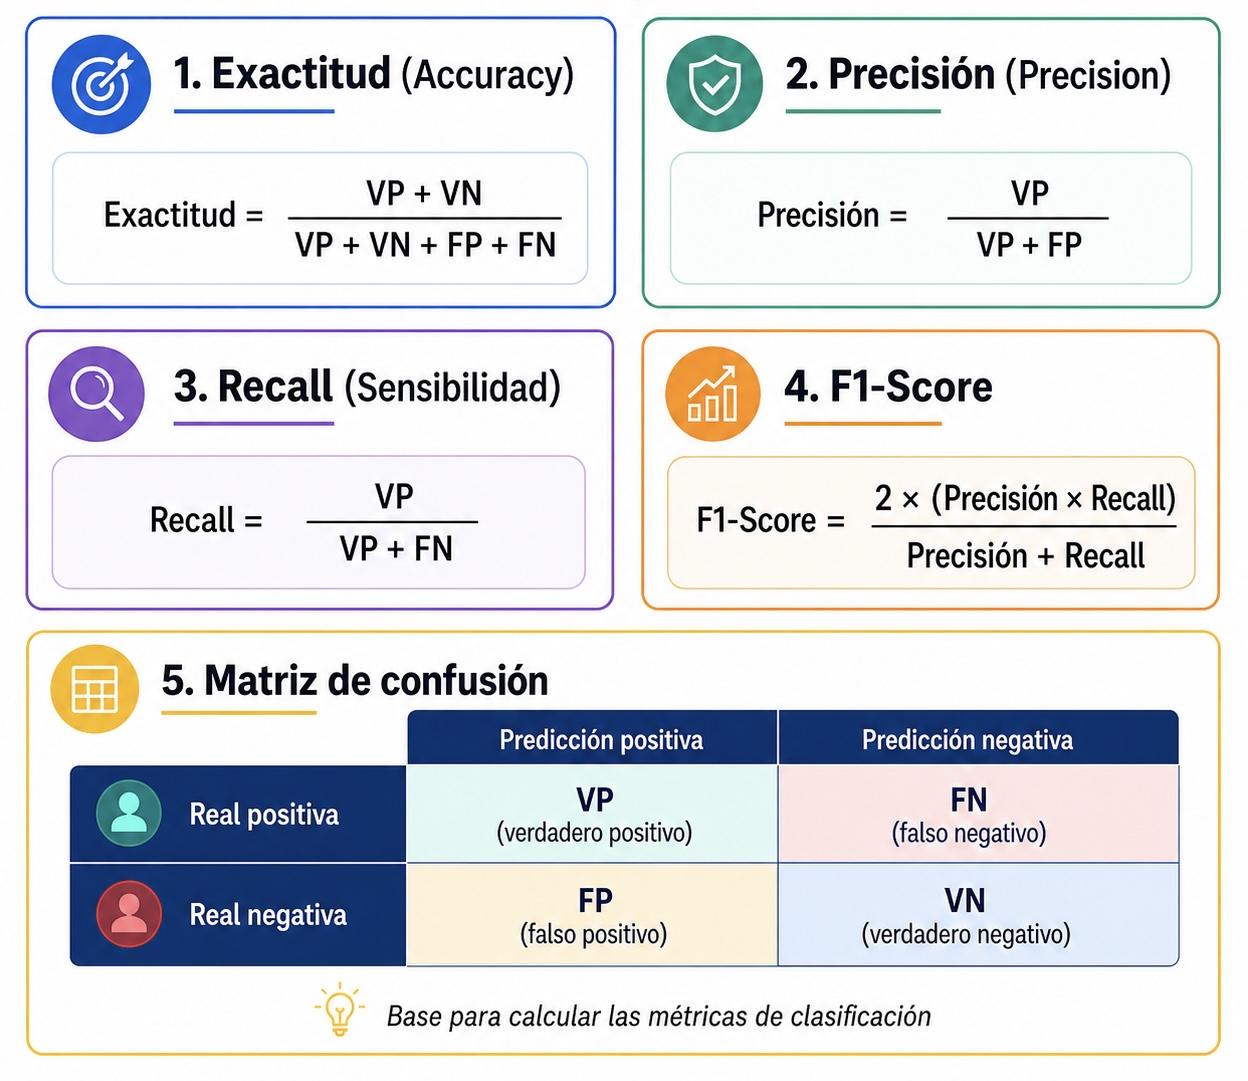
\includegraphics[width=0.8\textwidth]{images/C7/45EFD280-6BE0-4EC1-B893-7E16D4231F7E.jpeg}
    \caption{Métricas de evaluación del modelo de clasificación}
    \label{fig:metricasModelo}
\end{figure}


Estas métricas permiten determinar si el modelo es adecuado para apoyar la detección de posibles afectaciones por insectos descortezadores, considerando imágenes de corteza de arboles. 

\subsubsection{Métricas de desempeño del sistema}

El desempeño del sistema se evalúa considerando la respuesta de la aplicación móvil, la operación offline y el proceso de sincronización con la nube. Las métricas propuestas son:

\begin{itemize}
    \item \textbf{Tiempo de respuesta del análisis:} tiempo transcurrido desde que se captura o selecciona una imagen hasta que se muestra el resultado del análisis.
    \item \textbf{Tiempo de guardado local:} tiempo requerido para almacenar un análisis en la base local SQLite.
    \item \textbf{Tiempo de sincronización:} tiempo necesario para enviar registros pendientes desde la aplicación móvil hacia la nube.
    \item \textbf{Tasa de sincronización exitosa:} porcentaje de registros locales que se sincronizan correctamente.
    \item \textbf{Disponibilidad offline:} capacidad de la aplicación móvil para capturar, analizar y guardar registros sin conexión a internet.
    \item \textbf{Consistencia de datos:} verificación de que los registros sincronizados en la nube coincidan con los registros generados localmente.
\end{itemize}

Estas métricas permiten comprobar que el sistema cumple con el enfoque \textit{offline-first} y que la información generada en campo puede conservarse y sincronizarse correctamente.

\subsubsection{Criterios de aceptación del prototipo}

Los criterios de aceptación definen las condiciones mínimas que debe cumplir el prototipo para considerarse funcional. Para este proyecto se establecen los siguientes criterios:

\begin{itemize}
    \item El usuario puede iniciar sesión y acceder a las funciones correspondientes a su rol.
    \item La aplicación móvil permite capturar o importar imágenes para realizar análisis.
    \item El sistema permite seleccionar el tipo de análisis: follaje o corteza.
    \item Los análisis de corteza pueden asociarse a un árbol nuevo o existente.
    \item Los análisis de follaje pueden asociarse a una zona de monitoreo.
    \item El sistema genera un resultado de clasificación y un nivel de confianza.
    \item La aplicación almacena localmente los análisis realizados sin conexión a internet.
    \item Los registros pendientes se sincronizan con la nube cuando existe conexión disponible.
    \item La plataforma web permite consultar registros, mapas, historial y estadísticas consolidadas.
    \item La evidencia fotográfica puede consultarse desde la plataforma web después de la sincronización.
\end{itemize}

El cumplimiento de estos criterios permitirá validar que el prototipo cubre las funcionalidades esenciales definidas para el monitoreo forestal mediante aplicación móvil y plataforma web.